\chapter{Review of Reinforcement Learning}

\section{Introduction and terminology}
In section \ref{intro_rl} the RL framework was briefly discussed. In this chapter, the details of this methodology are explained.
\subsection{Markov Decision Process}
MDP is consecutive decision-making in which actions impact immediate rewards and later states, and hence future rewards. In other words, MDP is a stochastic control process using a discrete-time framework. An MDP system consist of 4 components (figure \ref{RL_agent}): 

\tikzstyle{block} = [rectangle, draw, 
text width=8em, text centered, rounded corners, minimum height=4em]

\tikzstyle{line} = [draw, -latex]
\begin{figure} 
	\centering
	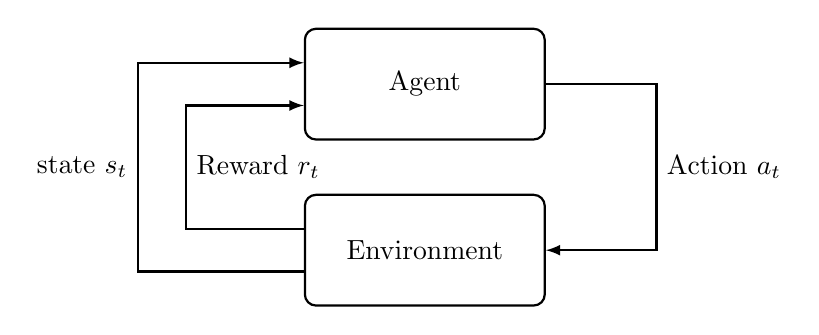
\begin{tikzpicture}[node distance = 6em, auto, thick]
		\node [block] (Agent) {Agent};
		\node [block, below of=Agent] (Environment) {Environment};
		
		\path [line] (Agent.0) --++ (4em,0em) |- node [near start]{Action $a_{t}$} (Environment.0);
		\path [line] (Environment.190) --++ (-6em,0em) |- node [near start] {state  $s_{t}$} (Agent.170);
		\path [line] (Environment.170) --++ (-4.25em,0em) |- node [near start, right] {Reward $r_{t}$} (Agent.190);
		\label{}
	\end{tikzpicture}
	\caption{Reinforcement learning schematic and the agent environment interaction.}
	\label{RL_agent}
\end{figure}

\begin{itemize}
	
	
	\item \textit{states} ($S_t \in \mathcal{S}$): A state (s) is a collection of all essential information about the current situation that can be used to forecast future states.  For example, in the case of a robot arm trying to grab a box, the current position of the robot arm could be the state. States can be a multidimensional discrete or continuous set. \\
	Sometimes, an observation of the states is available instead of the states themselves. For example, instead of a current position of the arm, a snapshot picture is available. 
	\item \textit{action} ($A_t \in \mathcal{A}$):   Actions are utilized to control the states by the agents \textit{policy}, which is a mapping from states to actions. It can be either stochastic $ a = \pi(.|s)$ or deterministic $a=\mu(s)$.  Actions somehow can be compared to the control input in the feedback of a control system. As an example, in a navigation problem, the actions are the torque applied to the wheels. Actions might belong to a discrete or continuous set, and they can also be multidimensional.
	\item \textit{Reward} ($R_t \in \mathcal{R} \subset \mathbb{R}$):  It is the measure of how well the agent is choosing the actions, to put it another way, how well is its \textit{policy}. For example, in the robot arm problem, it could be how close it is to grab the box.
	\item \textit{environment} $(p)$ : The environment is fully described by its \textit{dynamics} (distribution) which can be stochastic $s_{t+1} = p(.|s_t,a_t)$ or deterministic $s_{t+1} = p(s_t,a_t)$. Environment could be any sort of system in which a reward could be defined for a set of given actions applied to the environment. 	
	
\end{itemize}
The MDP framework is conceptual and adaptable, and it may be widely used in a variety of situations in several ways, including the stock price prediction \cite{lee2001stock} to low-level control of UAVs \cite{pi2020low}. Therefore, the definitions are different compared to a control platform. In an MDP, the interaction between the agent (controller) and the environment (the plant, controlled unit) happens in a discrete-time steps platform. The agent performs actions (control signal), receives the reward, and ends up being in a new state. Each interaction between the environment and the agent is called a \textit{step}. in each step the agent receives states $S_t$ and reward $R(s_t)$ from environment and generates a set of action(s) $A_t$  based on its policy which would transform the environment states to a new one $S_{t+1}$ based on transition probability $P(s_{t+1}|s_t,a_t)$ and consecutively provide with a $R_{t+1}$. So MDP can be defined as a tuple \cite{sutton2018reinforcement}:

\begin{equation}
	D\equiv (S, A, P, R)
\end{equation}
Expected Reward can be based on the current state and action $r = r(s,a)$:

\begin{equation}
	r(s,a) = \mathbb{E}[R_t|S_{t-1}=s,A_{t-1}]
\end{equation}
Or be based on the state-action-next state:

\begin{equation}
	r(s,a) = \mathbb{E}[R_t|S_{t-1}=s,A_{t-1},S_t=s']
\end{equation}
\subsubsection{Expected return}
Broadly speaking, the goal of a policy is to maximize the  average reward or discounted \textit{return} (a weighted average in which distant rewards have a less impact) in an episode\footnote{\textit{episode} consists of steps, starting from initial to terminal state, when the terminal state is reached, the process starts over from the initial state.}. In other words, the goal is to maximize the expected return $G_t$. There are different ways of defining the expected return \cite{kaelbling1996reinforcement}, here we discuss the one with discounted rate $\gamma \in (0,1)$ in an episode with T as final time step:\\

\begin{equation}
	G = R_{t}+\gamma R_{t+1}+ \gamma^2 R_{t+2}+ \dots + R_T\, \quad 0 \leq\gamma\leq 1 
\end{equation}

$\gamma$ is usually a number close to one since a low $\gamma$ can result in an instability \cite{kober2013reinforcement}. If $\gamma$ is chosen to be 1, then the approach is called average-reward criterion \cite{bertsekas2011dynamic}. In this case, it usually cannot distinguish between short-term transient reward, and it is mostly dominated by the steady-state region. If the policy achieves both acceptable short-term and long-term optimal behavior, then it is known as bias optimal \cite{lewis2002bias}. \\

\subsubsection{Value function}

The \textit{Value function} specifies how good a state is in an episode while a specific policy $\pi$ is followed. It can be based only on the state $V^\pi(s)$:
\begin{equation}
	\displaystyle V^\pi(s)= \mathbb{E}^{\pi}[G| s_t = s]
\end{equation}
where $\displaystyle \mathbb{E}_\pi$ denotes the expected return given that the agent follows policy. Note that the value of expected return should be calculated until terminal state is reached.
In a similar way the \textit{State-Action Value function} of acting $a$ in state (s) is defined as:
\begin{equation}
	\displaystyle Q^\pi(s,a)= \mathbb{E}^{\pi}[G|s_t=s,a_t=a]
\end{equation}

The value functions are policy dependent, meaning that the value of a state could be low in a policy while it would be high in another one; having this in mind, it is obvious that the optimal value functions are the ones obeying the optimal policy $\pi^*$:

\begin{equation}
	\displaystyle V^{\pi^*}(s)= \mathbb{E}^{\pi^*}[G| s_t = s]
\end{equation}

\begin{equation}
	\displaystyle Q^{\pi*}(s,a)= \mathbb{E}^{\pi^*}[G|s_t=s,a_t=a]
\end{equation}

$Q^{\pi*}(s,a)$ is the same as having the optimal policy because given the state (s) we can obtain the optimal policy from the below equation:

\begin{equation}
	a^*(s) =  \arg \max_a Q^*(s,a)
\end{equation}
\subsubsection{Bellman equation}
\textit{Bellman equation} expresses the value of a state, based on the value of its successor states. Bellman equation is obeyed in all the above equations for example in the Value function we have: 
\begin{equation}
	V^\pi(s_t) = R(s_t,\pi(s_t)) + \gamma \sum_{s_{t+1}} P(s_{t+1}|s_t,\pi(s_t)) V^\pi(s_{t+1}) 
\end{equation}

\begin{equation}
	V^{\pi^*}(s_t) = R(s_t,\pi^*(s_t)) + \gamma \sum_{s_{t+1}} P(s_{t+1}|s_t,\pi^*(s_t)) V^\pi(s_{t+1}) 
\end{equation}
In a situation with discrete actions, determining the optimal policy is simple, since an exhaustive search is possible if the optimal value function and the transition probabilities for the following states are known, however, in case of continuous spaces, function approximation methods are utilized.\\

There are numerous value function-based methods which has 3 major classes of:

\begin{enumerate}
	\item Dynamic programming-based methods.
	\item Monte Carlo methods
	\item Temporal difference methods.
\end{enumerate}

\subsection{Dynamic programming}

Dynamic Programming (DP) is well suited in a discrete scheme \cite{bucsoniu2010approximate}; however, it is possible to use it in a continuous framework. DP uses value functions to arrange and guide the search for optimal policies. The transition probability of the environment should be available, or it could be determined from experience.\\

In a DP algorithm \textit{policy iteration} is used, which is a process that alternates between \textit{policy evaluation} and \textit{policy improvement}. Initially, a random policy is used to start the approach, then the value function for the current policy is determined by policy evaluation. Each value of state in the current iteration is updated based on the values of the state in the previous iteration (bootstrapping), the policy $\pi$, and transition probability $p$. Finally, the policy is improved based on the most recent value function.

\subsection{Monte Carlo methods}

Unlike the DP, Monte Carlo methods learn directly from \textit{experience}\footnote{sampled episodes from environment} with no prior knowledge of MDP transitions. They carry out rollouts by executing the existing policy on the system, which is referred to as operating on-policy. The value function is updated after an episode is ended. This process is done using the average returns using the current experiences. The frequency of transitions and rewards is recorded and utilized to calculate value function estimates. As more episodes are produced, the average value will converge. The policy is improved by making it greedy regarding the value of the states. Although the method is quite simple, it is pretty powerful; for example, in the game of Tetris, this method outperforms most of the other ones \cite{gabillon2013approximate}.

\subsection{Temporal Difference}

Temporal Difference (TD) is a generalization of the Monte Carlo method. It also utilizes the bootstrapping of the DP so that TD(1) is the same as the Monte Carlo method, updating the values only when the episode is ended. TD(0) only considers the sampled successor states rather than the full distribution over the successor states in DP. In TD($\lambda$) ($0\geq\lambda\geq1$), values are updated before the end of the episode, and more than 1 step ahead is used.\\

Two popular TD approaches exist, with slightly different update procedures, state-action-reward-state-action (SARSA) \cite{rummery1994line}  and Q-learning \cite{watkins1992q}. SARSA uses the below equation for updating the Q value.

\begin{equation*}
	Q(s_t,a_t) \leftarrow Q(s_t,a_t) + \alpha [R_{t+1} + \gamma Q(x_{t+1},u_{t+1})-Q(s_t,u_t)]
\end{equation*}

While Q-learning uses:

\begin{equation}
	Q(s_t,a_t) \leftarrow Q(s_t,u_t) + \alpha [R_{t+1} + \gamma \max_{a_{t+1}} Q(x_{t+1},a_{t+1}) - Q(s_t,a_t)]
\end{equation}

SARSA is an on-policy algorithm, which means that its behavior and target policy are the same. Target policy is the output policy of the agent, which is used for evaluating the algorithm. The behavior policy $\pi_b$ is how the agent acts in exploration. Since exploratory policies are not optimal, \textit{on-policy} methods such as SARSA may quickly converge to a local optimum.\\

\textit{Off-policy} agents, such as Q-learning, employ different target and behavior policies; hence, they may use equal probability for taking actions in each state, so $\pi_b(a^*|s)>0$; as a result, they would find the optimal policy given enough time \cite{sutton1988learning}.\\

Value function methods struggle with the challenges of RL in robotic because they demand data to be filled into the entire state-action space, and they are intrinsically unstable \cite{szepesvari2010algorithms}. In addition, the bootstrapping will result in a bias if we want to use function approximation techniques which is inevitable in continuous spaces of robotics. As a result, value-based methods are not suitable for robotic applications, so we introduce a new family of RL methods called the policy search in the next section.

\section{Policy search}

Policy search approaches do not require using a value function model and instead search for the optimal policy. The concept behind this method is that it is feasible to enhance an episode's return without knowing the value of each state. The disadvantage of this technique is that it requires evaluating the policy and calculating the return in order to determine if the chosen policy is superior or not. Usually, a parameterized policy is chosen, and the parameters are tuned to maximize the expected return. This is usually done by methods such as gradient ascent \cite{baird1999reinforcement} or hill climbing \cite{kimura1995reinforcement}. \\

Policy searches provide many advantages. For example, it is feasible to take advantage of an expert for parameter initialization \cite{peters2006policy}, or it is possible to choose the suitable policy parameter structure, ensuring robustness and stability \cite{bertsekas2011dynamic}. Therefore, making policy search, a well-suited method for robotic which is proven by real system applications \cite{deisenroth2014multi, vikas2015model}.\\

In the case where gradient ascent is used for the optimization of the policy, we have: 
\begin{equation}
	J(\pi_{\kappa}) = \mathbb{E}^{\pi_{\kappa}}[G_{t}]
\end{equation}
\begin{equation}
	\kappa_{k+1}=\kappa_k+\alpha (\nabla_{\kappa} J(\pi_{\kappa})|_{\kappa=\kappa_k}
\end{equation}
In which, $\nabla_{\kappa} G_{\pi_{\kappa}}|$ is called \textit{policy gradient} \cite{sutton1999policy}. Which can be expressed as:

\begin{equation}
	\nabla_{\kappa} J_{\pi_{\kappa}} = \gamma^t G_{t}  \frac{\nabla_{\kappa} \pi_{\kappa}(a_t|s_t)}{\pi_{\kappa}(a_t|s_t)}
\end{equation}

\begin{equation}
	\nabla_{\kappa} J_{\pi_{\kappa}} = \gamma^t G_{t} \nabla_{\kappa}   \log \pi_{\kappa}(a_t|s_t) 
	\label{reinforce equation}
\end{equation}
The term $\nabla_{\kappa}   \log \pi_{\kappa}(a_t|s_t)$ is referred to as \textit{eligibility vector}.
Equation \ref{reinforce equation} is first introduced by \cite{williams1992simple} known as REINFORCE algorithm. This algorithm needs the episode to be terminated to calculate $G_t$, which is why this algorithm is considered a Monte Carlo algorithm. Methods such as Trusted Region Policy Optimization (TRPO) \cite{schulman2015trust} or Proximal Policy Optimization (PPO) \cite{schulman2017proximal} are examples of using such methodology.\\

For continuous actions, instead of learning the probability of the infinite number of actions, usually a Gaussian distribution is used:

\begin{equation}
	\pi(a|s,\kappa) = \frac{1}{a_\sigma(s,\kappa) \sqrt{2\pi}} exp\big( -\frac{(a-a_\mu(s,\kappa))^2}{2a_\sigma(s,\kappa)^2} \big)
\end{equation}

One of the methods to parameterize the policy is using a neural network named Deep Reinforcement Learning.

\subsection{Deep Reinforcement Learning}

In RL, neural networks (NN) are function approximation tools when the state or action space is continuous or too large. In some instances, it is simpler to approximate the value function, whereas, in others, it is easier to approximate policy. In latter cases, policy-based methods are more favorable as they yield a better asymptotic policy \cite{simsek2016most}. In both cases, a neural network can be employed for value approximation or policy approximation.\\

Neural networks can learn to map states to values or state-action pairs to Q values. Instead of using a lookup table to store, index, and update all possible states and their values - which is impossible with huge problems- We can train a neural network on samples from the state and action space to predict the value of states or which actions to take given a state.\\

Now that policy search is introduced, it is possible to discuss the next generation of RL, actor-critic methods.\\

\section{Actor-critic methods}

Actor-critic methods are policy search methods in which a bias is introduced through bootstrapping in order to improve learning speed and reduce variance. The actor-critic method to the REINFORCE is like the TD algorithm to the Monte Carlo methods. \\

If only one step of the return is considered, (like TD(0)) the general formula for an actor-critic method can be given as:
\begin{equation}
	\kappa_{k+1}=\kappa_k+\alpha \big(R_{t+1}+\gamma \hat{v}_\omega (S_{t+1})-\hat{v}_\omega(S_t)\big) \nabla_{\kappa}   \log \pi_{\kappa}(a_t|s_t)
\end{equation}

\section{Soft Actor Critic} \label{sacsection}

%DDPG, an algorithm that concurrently learns a deterministic policy and a Q-function by using each to improve the other, and SAC, a variant that uses stochastic policies, entropy regularization, and a few other tricks to stabilize learning and score higher than DDPG on standard benchmarks.
Soft Actor-Critic (SAC) is an actor-critic off-policy algorithm with a stochastic policy \cite{haarnoja2019soft,haarnoja2018soft}. It is inspired by stochastic policy optimization and Deep Deterministic Policy Gradient (DDPG) approaches \cite{lillicrap2015continuous}. It has similarities to Twin Delayed DDPG (TD3)  method \cite{fujimoto2018addressing} such that both use two clipped Q approximators. Since it is a stochastic method, it also benefits from something similar to target policy smoothing. Which makes it a potent tool in the robotic control field \cite{haarnoja2019learning}.\\


The main feature of the SAC algorithm is that it tries to balance a trade-off between expected return and entropy \cite{gray2011entropy}. The more the entropy, the higher the exploration, and the less the entropy, the higher the expected return in the short term. This is related to the exploration-exploitation trade-off: increasing entropy leads to more exploration, speeding up learning later. It can also prevent converging to futile local optimums.\\

Before we can discuss the further details of the algorithm, it is necessary to discuss the details of the usage of entropy in RL.
\subsection{Entropy-Regularized Reinforcement Learning}
The entropy-regularized reinforcement learning changes the goal of RL by including an entropy term, so that the optimal policy not only aims to increase the reward but also tries to increase its entropy at each visited state \cite{haarnoja2017reinforcement}. The temperature parameter $\alpha$ balance between exploration and exploitation in such way that by increasing $\alpha$ the policy would try to explore more by adding a stochastic term the reward importance. The formula for this method is:

\begin{equation}
	\pi^* = \arg \max_\pi \mathbb{E}_{\tau \sim \pi} [\sum_{t=0}^{T} \gamma^t \big( r(s_t,a_t,s_{t+1}) + \alpha H(\pi(.|s_t)) \big)]
\end{equation}

in which $H(\pi(.|s_t))$ is the entropy of a stochastic policy, given by:

\begin{equation}
	H(\pi(.|s_t)) =  \mathbb{E}[-\log \pi(.|s_t)]
\end{equation}

So, comparing a deterministic policy to an entropy regularized policy, when multiple actions are almost equally valuable, the policy commits equal probability mass to the actions instead of choosing the most valuable action. In this framework, the state value and the state-action value should be modified:

\begin{equation}
	V_\pi(s) = \mathbb{E}_{\tau \sim \pi}\Bigg[\sum_{t=0}^{T} \gamma^t \bigg( r\Big(s_t,a_t,s_{t+1}+\alpha H\big(\pi(.|s_t)\big)\Big) \bigg)|s_0=s\Bigg]
\end{equation}

\begin{equation}
	Q_\pi(s) =  \underset{\tau \sim \pi}{\mathbb{E}}\Bigg[\sum_{t=0}^{T} \gamma^t \bigg( r\Big(s_t,a_t,s_{t+1}+\alpha H\big(\pi(.|s_t)\big)\Big) \bigg)|s_0=s, a_0=a\Bigg]
\end{equation}

\subsection{SAC algorithm}

The SAC algorithm is given in Algorithm \ref{sac algorithm}. The Q functions are updated using the Mean Squared Bellman Error (MSBE)\\

\begin{equation}
	L(\delta_i, {\mathcal D}) = \underset{(s,a,r,s_{t+1},d) \sim {\mathcal D}}{{\mathbb{E}}}\left[
	\Bigg( Q_{\delta_i}(s,a) -  \underbrace{\big(r + \gamma \min Q_{\delta_{targ,j}}(s_{t+1}, a_{t+1}) - \alpha \log \pi_{\kappa}(a_{t+1}|s_{t+1})\big)}_{y(r,s_{t+1},d)} \Bigg)^2
	\right],
\end{equation}

In which D is the buffer of the algorithm in which the transitions are stored.
Hence the Q functions are updated by the following gradient:
\begin{align}
	& \delta_{i,new} = \delta_{i,old}+ l_{\delta} \nabla_{\delta_{i,old}} \frac{1}{|B|}\sum_{(s,a,r,s_{t+1},d) \in B} \left( Q_{\delta_{i,old}}(s,a) - y(r,s_{t+1},d) \right)^2 && \text{for } i=1,2
\end{align}
The policy is updated given:
\begin{equation}
	\max_{\kappa} \underset{s \sim \mathcal{D}, \xi \sim \mathcal{N}}{\mathbb{E}}{\min Q_{\delta_i}(s,a_{\kappa}(s,\xi)) - \alpha \log \pi_{\kappa}(a_{\kappa}(s,\xi)|s)},
\end{equation}
The policy is updated by:
\begin{equation}
	\kappa_{new}=\kappa_{old} + l_{\kappa}\nabla_{\kappa} \frac{1}{|\mathcal{B}|}\sum_{s \in \mathcal{B}} \Big(\min Q_{\delta_i}(s, a_{\kappa}(s)) - \alpha \log \pi_{\kappa} \left(\left. a_{\kappa}(s) \right| s\right) \Big)
\end{equation}
sampling $a_{\kappa}(s)$ from Gaussian distribution of policy $\pi_{\kappa}(\cdot|s)$ is done by the squashed Gaussian function:
\begin{equation}
	a_t = f_\kappa (s_t, \xi_t)
\end{equation}
\begin{equation}
	a_t = tanh(\mu_\kappa(s_t)+\sigma_\kappa(s_t) \cdot \xi_t), \quad \quad \xi \in \mathcal{N} (0,I)
\end{equation}
However, after convergence is reached in order to evaluate the policy, the randomness term of the action is omitted to improve performance:
\begin{equation}
	\bar{a}_t = tanh(\mu_\kappa(s_t))
\end{equation}

\newpage
\begin{algorithm}[H]
	\caption{Soft Actor-Critic}
	\label{alg1}
	\begin{algorithmic}[1]
		\STATE \textbf{Initialization}: initialize policy parameters $\theta$
		\STATE initialize Q-function parameters $\delta_1$, $\delta_2$
		\STATE initialize target network parameters $\delta_{\text{targ},1} \leftarrow \delta_1$, $\delta_{\text{targ},2} \leftarrow \delta_2$
		\STATE initializing the replay pool $\mathcal{D}$
		\REPEAT
		\REPEAT
		\STATE  sample action $a \sim \pi_{\theta}(\cdot|s)$ 
		\STATE observe next state $s_{t+1}$ reward $r$ and done signal $d  \in [\text{TRUE},\text{FALSE}]$
		\STATE save $(s_t,a_t,r(s_t,a_t),s_{t+1},d)$ in replay pool $\mathcal{D}$
		\IF  {d is \textbf{TRUE}}
		\STATE reset environment state.
		\ENDIF
		\UNTIL{ $\mathcal{D}>\mathcal{D}_{min}$}
		\STATE  sample action $a \sim \pi_{\theta}(\cdot|s)$ 
		\STATE observe next state $s_{t+1}$ reward $r$ and done signal $d  \in [\text{TRUE},\text{FALSE}]$
		\STATE save $(s_t,a_t,r(s_t,a_t),s_{t+1},d)$ in replay pool $\mathcal{D}$
		\IF  {d is \textbf{TRUE}}
		\STATE reset environment state.
		\ENDIF
		\IF{it's time to update the parameters}
		\FOR{$j$ in range(however many updates)}
		\STATE sample a batch of transitions, $\mathcal{B} = \{ (s,a,r,s_{t+1},d) \}$ from $\mathcal{D}$
		\STATE Update Q-functions.
		\STATE Update policy.
		\STATE Update target networks by linearization 
		\begin{align*}
			\delta_{\text{targ},i} &\leftarrow \eta \delta_{\text{targ}, i} + (1-\eta) \delta_i && \text{for } i=1,2 \\
		\kappa_{\text{targ}}&\leftarrow \eta \kappa_{\text{targ}} + (1-\eta) \kappa
		\end{align*}
		\ENDFOR
		\ENDIF
		\STATE evaluate the policy to check the convergence using $\bar{a}_t$
		\UNTIL {convergence}
		\STATE \textbf{Return} $\kappa, \delta_1$ and $\delta_2$
	\end{algorithmic}
	\caption{sac algorithm}
	\label{sac algorithm}
\end{algorithm}
